Wie tief dringen Teilchen in das Detektormaterial ein? Man kann für jede
Projektil/Target-Kombination nur eine mittlere Eindringtiefe angeben. Der Energieverlust eines
Projektils in Abhängigkeit von der Eindringtiefe wird durch die Bragg-Kurve beschrieben. Mit
Eindringen in die Materie wird das Projektil langsamer, der Energieverlust steigt an
(Bethe-Bloch). Die Reichweite $R$ enthält man aus der Integration des Energieverlustes entlang des
Weges, wobei $\frac{dE}{dx}$ hierbei eine Funktion von $E$ ist. Bei ionisierender Strahlung kommt es
am Ende der Reichweite wegen $\frac{1}{\beta^2}$-Verhalten zu einer besonders hohen Dichte der
deponierten Energie.

\[dE= \frac{dE}{dx}(E)dx~~~~~~~~~~\Rightarrow~~~~~~~~~~dx
=\frac{dE}{dE/dx}~~~~~~~~~~\Rightarrow~~~~~~~~~~ R=\int_{E_c}^{M} \frac{dE}{dE/dx}  \]

Der größte Ionisationsverlust findet nahe am Ende der Spur statt (Bragg-Peak).



% Absorptionsprozesse (mit $dN=8\mu dx$) führen zu einem exponentiellen Abfall der Teilchenzahl.

% \begin{figure}
% \begin{minipage}{0.45\textwidth}
% 
% \end{minipage}
% \begin{minipage}{0.45\textwidth}
% 
% \end{minipage}
% \caption{bla}
% \end{figure} 

\begin{figure}[htbp]
	\begin{minipage}[b]{0.5\textwidth}
		\begin{figure}[H]
		\centering
		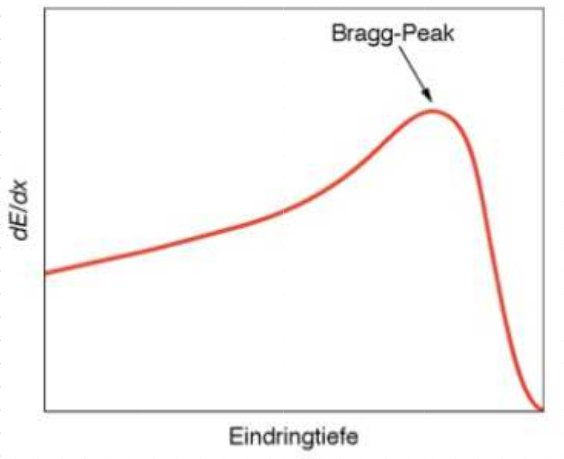
\includegraphics[width=\textwidth]{bragg.jpg}
		\end{figure}
	\end{minipage}
	\hfill
	\begin{minipage}[b]{0.5\textwidth}
		\begin{figure}[H]
		\centering
		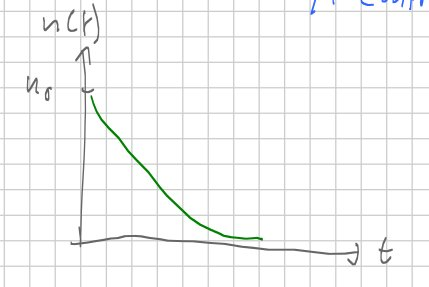
\includegraphics[width=\textwidth]{expabfall.jpg}
		\end{figure}
	\end{minipage}
	\caption{b}
	\label{rekristall} 
\end{figure}